I contenuti multimediali sono diffusi su Internet tramite il World Wide Web, un servizio Internet semplice ed efficace che usa protocolli di livello applicativo.
\\
Fin dalle origini del Web, l'approccio tipico e stato l'uso di server centralizzati (origin server) nella rete backbone. Questo comporta un problema importante: i client che accedono allo stesso contenuto generano un carico molto elevato sui server e sulla rete, soprattutto con il forte aumento del traffico Internet nell'ultimo decennio.
\\
Questo carico può essere ridistribuito meglio usando strategie e dispositivi specificamente progettati per gestire l'aumento di traffico. Inoltre, tali strategie permettono di ottenere latenze ridotte e un uso piu efficiente delle risorse.
\begin{figure}[H]
	\centering
	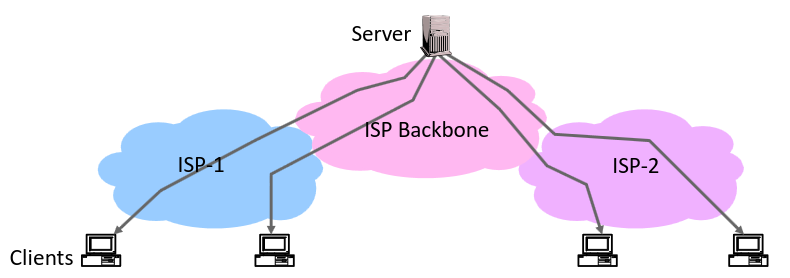
\includegraphics[width=0.8\textwidth]{pictures/7/rete.png}
	\caption{Esempio di distribuzione dei contenuti tramite CDN.}
\end{figure}
\section{Uso dei proxy}
Un \textbf{proxy} è un dispositivo di livello applicativo che replica contenuti e si colloca tra client e origin server. In questo modo, la distribuzione dei contenuti migliora.
\\
Le principali possibilita sono due:
\begin{itemize}
	\item adozione di \textbf{reverse proxy};
	\item adozione di \textbf{forward proxy}.
\end{itemize}
\begin{figure}[H]
	\centering
	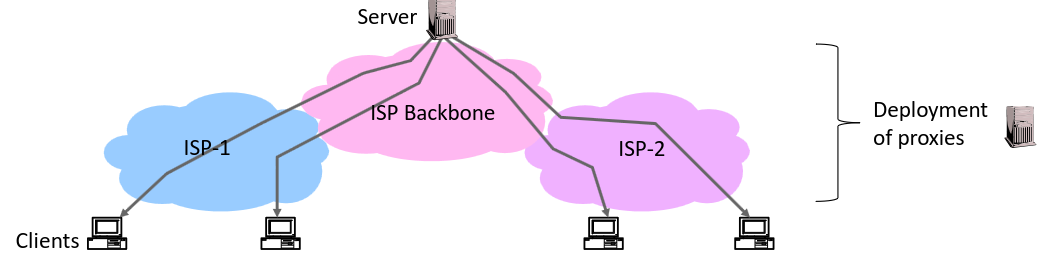
\includegraphics[width=0.8\textwidth]{pictures/7/proxy.png}
	\caption{Esempio di uso di proxy.}
\end{figure}
\subsection{Reverse proxy}
I reverse proxy sono un insieme di server front-end dell'origin server, usati per ridurne il carico e collocati comunque nel backbone.
\\
È necessario eseguire il load balancing tra i reverse proxy. L'utilizzo di reverse proxy non allieva in modo significativo il carico sulla rete.
\begin{figure}[H]
	\centering
	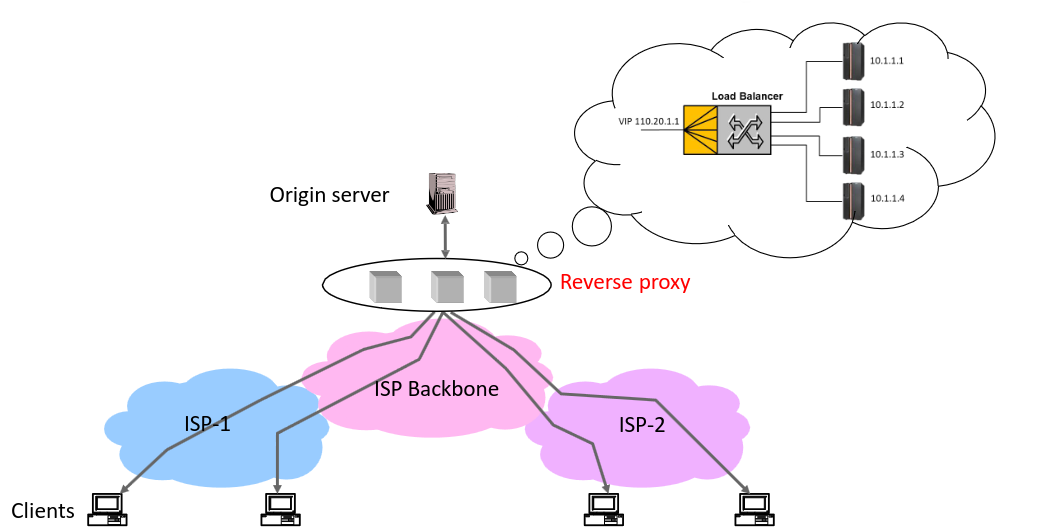
\includegraphics[width=0.8\textwidth]{pictures/7/reverseProxy.png}
	\caption{Esempio di uso di reverse proxy.}
\end{figure}
\subsection{Forward proxy}
I forward proxy sono posti vicino ai client.
\begin{itemize}
	\item Possono essere distribuiti nelle reti private aziendali o nelle reti ISP.
	\item Replicano localmente i contenuti.
	\item Il load balancing è necessario solo se esistono piu forward proxy locali.
\end{itemize}
Data la loro posizione, i forward proxy riducono il carico di rete se la replica dei contenuti e effettuata in modo intelligente. Inoltre, si osserva una riduzione della latenza nel recupero dei contenuti replicati.
\\
D'ora in avanti, forward e reverse proxy verranno indicati con il termine generico \textbf{cache} (o \textbf{replica server}).
\begin{figure}[H]
	\centering
	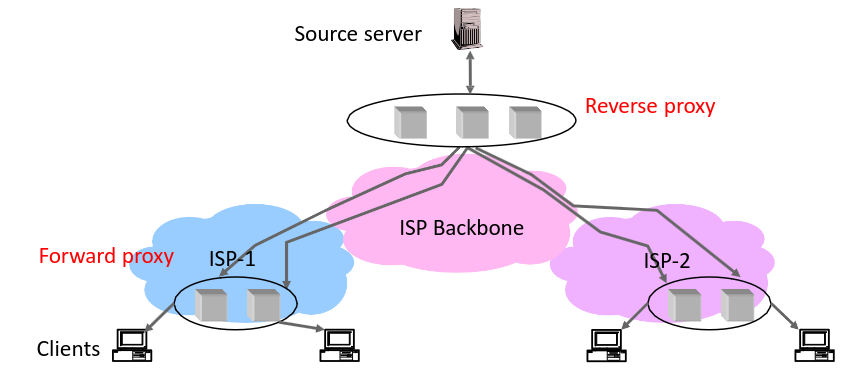
\includegraphics[width=0.8\textwidth]{pictures/7/forwardProxy.png}
	\caption{Esempio di uso di forward proxy.}
\end{figure}
\section{Replica dei contenuti (caching)}
La capacità di memoria delle cache vicine agli utenti è limitata.
\\
Una strategia di caching consiste nel replicare i contenuti popolari.
È quindi necessario definire cosa si intende per \emph{popolare}:
in genere, i contenuti più frequentemente acceduti.
La logica di questa strategia è che una piccola quantità di contenuti molto popolari
genera una percentuale molto elevata di accessi.
\\
La popolarità di un contenuto può essere espressa come:
\[
\text{Popolarita}(m)=\frac{\#\,\text{accessi al contenuto }m}{\#\,\text{accessi totali}}
\]

Un modello tipico e la funzione di Zipf:
\[
h(m)=\frac{K}{m^{\phi}}
\]

Dove spesso una quota ridotta dei contenuti genera la maggior parte degli accessi (principio 80/20).
\begin{figure}[H]
	\centering
	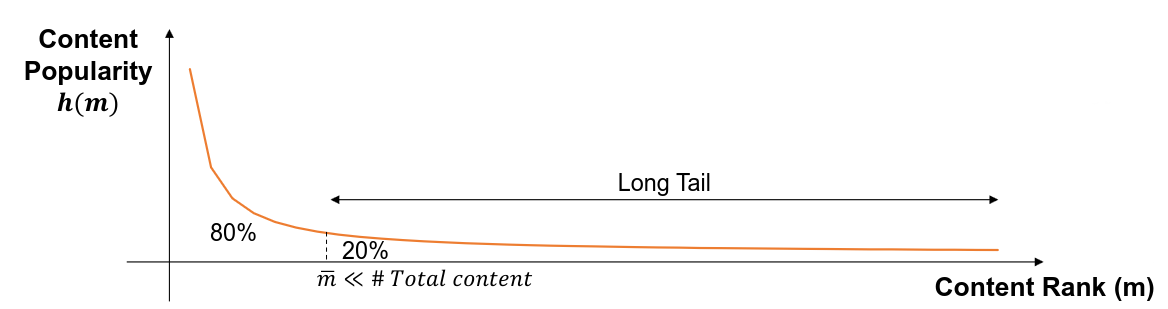
\includegraphics[width=\textwidth]{pictures/7/popolarità.png}
	\caption{Esempio di distribuzione della popolarità dei contenuti secondo la funzione di Zipf.}
\end{figure}
\subsection{Localita degli accessi}
Gli accessi ai contenuti mostrano spesso correlazione di localita, sfruttata dal caching:
\begin{itemize}
	\item \textbf{Localita temporale}: un contenuto acceduto in un certo istante è probabilmente acceduto di nuovo dopo poco tempo.
	\item \textbf{Localita spaziale}: un contenuto acceduto in un'area geografica è probabile che venga acceduto anche in aree geografiche vicine.
\end{itemize}

\section{Il problema della consistenza}
La \textbf{consistenza} e la proprieta che garantisce l'allineamento delle repliche: in linea di principio, la stessa versione del contenuto dovrebbe essere presente in tutti i replica server.
\\
Esistono due gradi di consistenza:
\begin{itemize}
	\item \textbf{forte}: evita la consegna di repliche inconsistenti agli utenti;
	\item \textbf{debole}: è possibile che gli utenti ricevano repliche inconsistenti, ma con bassa probabilità.
\end{itemize}
Per garantire consistenza si usano tre meccanismi:
\begin{itemize}
	\item \textbf{Invalidation}: le repliche sono invalidate dopo la scadenza del \emph{tempo di scadenza atteso} definito dall'origin server.
	\item \textbf{Freshness}: garantisce che una replica possa essere considerata \emph{fresca} (non obsoleta); serve perche un contenuto puo cambiare anche prima del tempo di scadenza atteso.
	\item \textbf{Validation}: verifica se una replica è ancora valida anche dopo la scadenza del tempo atteso.
\end{itemize}

\section{Cooperative caching}
\raggedcolumns
\begin{multicols}{2}
Quando una cache non contiene un contenuto richiesto (\emph{cache miss}), puo richiederlo ad altre cache invece che all'origin server.

Esistono due tipi di cooperative caching:
\begin{itemize}
	\item \textbf{flat}: tutte le cache sono allo stesso livello;
	\item \textbf{gerarchico}: le cache sono organizzate gerarchicamente.
\end{itemize}

Nel caso gerarchico la distribuzione dei contenuti e organizzata ad albero, e i contenuti replicati possono essere richiesti solo al nodo padre.

\columnbreak

% L'immagine occupa soltanto la colonna destra (nessun float all'interno delle colonne)
\vspace{0pt}\begin{center}
	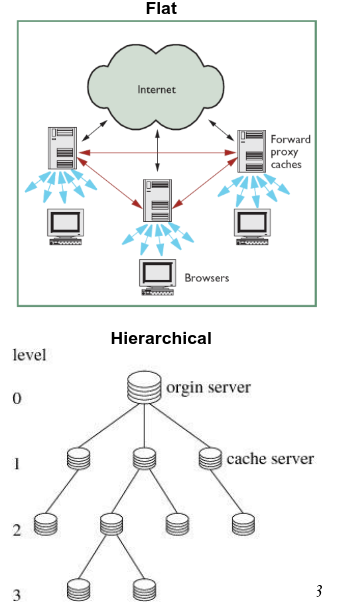
\includegraphics[width=0.9\linewidth]{pictures/7/cooperativeCaching.png}
\end{center}
\end{multicols}
\section{Direttive HTML e HTTP}
Il linguaggio HTML e il protocollo applicativo HTTP consentono a client e server di specificare le modalità di caching di un contenuto tramite funzioni dette \textbf{direttive}.
\subsection{Direttive HTML}
Vengono inserite direttamente nel codice HTML della pagina web, dunque sono
facili da controllare per i webmaster.
D'altro canto, sono limitate alle pagine scritte in HTML.
\\
Esempio:
\begin{verbatim}
<meta http-equiv="pragma" content="no-cache">
\end{verbatim}
\noindent
Questa meta direttiva forza il recupero della pagina dall'origin server.

\subsection{Direttive HTTP}
Implementate tramite campi di intestazione nelle richieste/risposte HTTP.
Sono più facili da gestire nei sistemi di caching e più diffuse.
\\
Esempi: \texttt{Cache-control:}, \texttt{Expires:}, \texttt{If-modified-since:}.
\\
Formato generale di una richiesta HTTP:
\begin{verbatim}
GET <contenuto> HTTP/1.1
<chiave1>: <valore1>
<chiave2>: <valore2>
...
<message body>
\end{verbatim}
Dove \texttt{<chiave>: <valore>} rappresenta un campo di intestazione (header) che specifica una direttiva HTTP.
\section{Direttive HTTP imperative}
Hanno priorità sugli altri controlli eseguiti dalle cache.
\\
Direttive in richieste e risposte:
\begin{itemize}
	\item \texttt{Cache-control: no-store}: impedisce il caching del contenuto.
	\item \texttt{Cache-control: no-transform}: impedisce alla cache di trasformare il contenuto (ad esempio transcoding).
\end{itemize}
\noindent
Direttive solo nelle richieste:
\begin{itemize}
	\item \texttt{Cache-control: only-if-cached}: richiede l'uso esclusivo di contenuto in cache.
\end{itemize}
\noindent
Se il contenuto non e in cache, la cache risponde con l'errore \texttt{504 Gateway Timeout}.

\section{Direttive HTTP per il ciclo di vita del contenuto}
\begin{itemize}
	\item \texttt{Date}: istante in cui il contenuto e stato inviato dall'origin server alla cache.
	\item \texttt{Last-modified}: ultimo istante di modifica del contenuto da parte dell'origin server.
	\item \texttt{Age}: tempo trascorso dall'oggetto in cache.
	\item \texttt{Expires}: previsione del server su quando le copie devono essere sostituite (tempo di scadenza atteso).
\end{itemize}
\begin{figure}[H]
	\centering
	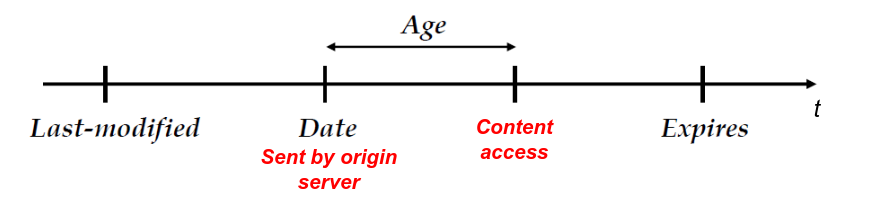
\includegraphics[width=0.8\textwidth]{pictures/7/lifecycle.png}
	\caption{Esempio di ciclo di vita del contenuto.}
\end{figure}
Condizioni indicate:
\begin{itemize}
	\item Se \texttt{Last-modified < Date}, la replica e consistente.
	\item Se \texttt{Date + Age < Expires}, il contenuto e valido.
\end{itemize}

\section{Direttive HTTP temporali}
\begin{figure}[H]
	\centering
	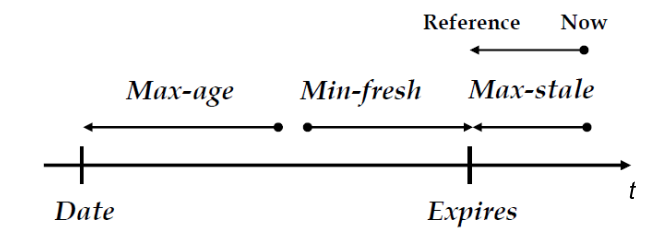
\includegraphics[width=0.6\textwidth]{pictures/7/temporal.png}
	\caption{Esempio di direttive HTTP temporali.}
\end{figure}
I client possono richiedere contenuti con requisiti temporali.
\begin{itemize}
	\item \texttt{Max-age}: il client accetta contenuto con età non superiore al valore specificato.
	\item \texttt{Min-fresh}: il client accetta contenuto che resterà \emph{fresco} (lontano da \texttt{Expires}) almeno per il tempo specificato.
	\item \texttt{Max-stale}: il client può accettare contenuto un po' obsoleto (cioè oltre \texttt{Expires}).
\end{itemize}
\noindent
Per impostazione predefinita, le cache non restituiscono contenuti obsoleti (\texttt{Max-stale} non specificato).

\subsection{Tempo di scadenza previsto dal server}
Il valore indicato in \texttt{Expires} e una previsione dell'origin server e può essere errata.
\\
Se è possibile garantire che l'origin server non modifichi un oggetto prima del tempo di scadenza atteso, si ottiene consistenza forte.
\\
Il meccanismo di validazione viene usato quando il tempo di scadenza atteso e raggiunto.

\section{Validazione dal lato client}
Il client cerca una replica valida del contenuto.
\\
La validazione è il processo di verifica svolto dalla cache, con il coinvolgimento dell'origin server, con l'obiettivo di capire se una replica è ancora utilizzabile dopo la scadenza.
\\
Flusso operativo:
\begin{enumerate}
	\item La cache invia una richiesta GET con uno dei seguenti campi:
	\begin{itemize}
		\item \texttt{If-none-match: <Etag della replica in cache>}
		\item \texttt{If-modified-since: <data della replica in cache>} (usato se il contenuto non ha Etag)
	\end{itemize}
	\item Il server risponde con:
	\begin{itemize}
		\item se l'oggetto è stato modificato: nuovo oggetto, risposta \texttt{HTTP/1.0 200 OK};
		\item se l'oggetto non è stato modificato: risposta \texttt{HTTP/1.0 304 Not Modified}.
	\end{itemize}
\end{enumerate}

\texttt{Etag} è una stringa univoca che distingue versioni diverse di uno stesso contenuto.
\begin{figure}[H]
	\centering
	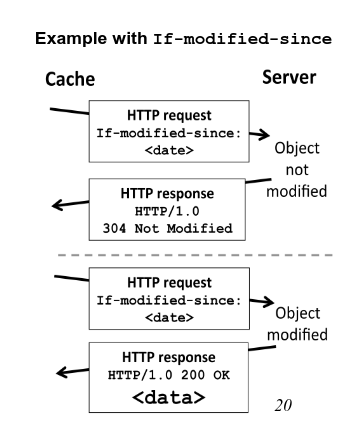
\includegraphics[width=0.4\textwidth]{pictures/7/modified.png}
	\caption{Esempio di validazione dal lato client.}
\end{figure}

Esempio con \texttt{If-none-match}:
\begin{verbatim}
GET /img/ietf.png HTTP/1.1
[...]
If-none-match: "aa0b06-754-4a29893aa8fc0"

HTTP/1.1 304 Not Modified
[...]
Date: Tue, 12 May 2022 05:21:29 GMT
Etag: "aa0b06-754-4a29893aa8fc0"
\end{verbatim}

\section{Eterogeneita dei contenuti}
Esistono contenuti eterogenei:
\begin{itemize}
	\item \textbf{Statici}: abbastanza stabili nel tempo (es. pagine HTML, archivi, contenuti multimediali).
	\item \textbf{Volatili}: cambiano frequentemente, periodicamente o per eventi in corso (es. news, eventi sportivi, titoli di borsa).
	\item \textbf{Dinamici}: creati dinamicamente in base alla richiesta del client (es. motori di ricerca, e-commerce).
\end{itemize}

\subsection{Quali contenuti replicare}
Una parte significativa dei contenuti Internet (oltre il 50\%) e \emph{non cachabile}.
\\
Cause principali della non-cachabilita:
\begin{itemize}
	\item \textbf{Volatilita}: variazioni frequenti nel tempo rendono costoso allineare le repliche.
	\item \textbf{Dinamicita}: le cache in genere non sono progettate per generare contenuti dinamici.
	\item \textbf{Cifratura}: i dati cifrati non sono cachabili.
	\item \textbf{Advertising/Analytics}: ad esempio, il proprietario di un banner vuole tracciare il numero di click.
\end{itemize}
\noindent
Osservazioni:
\begin{itemize}
	\item gran parte dei contenuti volatili o dinamici ha dimensione piccola, quindi ha impatto ridotto sul carico di rete;
	\item i contenuti statici hanno tipicamente dimensioni maggiori, quindi impatto significativo sul carico di rete.
\end{itemize}
\noindent
Di conseguenza, i contenuti statici sono quelli maggiormente soggetti a caching.
\section{Content Delivery Network (CDN)}
Una CDN garantisce una distribuzione intelligente dei contenuti offerti dal \textbf{Content Provider}, proprietario dell'origin server.
\\
È un'infrastruttura creata per distribuire efficientemente tali contenuti agli utenti, includendo molte cache disseminate nella rete dal \textbf{CDN Provider}.
\\
Modello di business tipico:
\begin{itemize}
	\item il CDN Provider stipula accordi con Network Operator (es. ISP) per il posizionamento delle cache nelle loro reti;
	\item il servizio CDN è offerto dai CDN Provider ai Content Provider che hanno contenuti popolari da distribuire.
\end{itemize}
\noindent
Gli obiettivi prestazionali del servizio CDN sono:
\begin{itemize}
	\item ridurre la latenza di accesso ai contenuti (beneficio per i Content Provider);
	\item ridurre la banda di rete consumata (beneficio per i Network Operator).
\end{itemize}

\section{Architettura di una CDN}
Componenti di content delivery:
\begin{itemize}
	\item origin server;
	\item replica server (cache).
	\item Sistema di distribuzione dei contenuti
	\begin{itemize}
		\item Replica i contenuti dell'origin server nei replica server.
		\item Garantisce la consistenza.
		\item Si basa sui principi di caching visti in precedenza.
	\end{itemize}
	\item Sistema di instradamento delle richieste
	\begin{itemize}
		\item Instrada le richieste degli utenti verso un server (origin oppure replica).
	\end{itemize}
	\item Sistema di accounting
	\begin{itemize}
		\item Mantiene i log di accesso degli utenti.
		\item Esegue analisi del traffico.
		\item Consente ai Content Provider di addebitare gli utenti.
		\item Si interfaccia con i sistemi di billing dei Content Provider.
		\item Puo essere consultato (previa autenticazione) da più Content Provider.
	\end{itemize}
\end{itemize}
\begin{figure}[H]
	\centering
	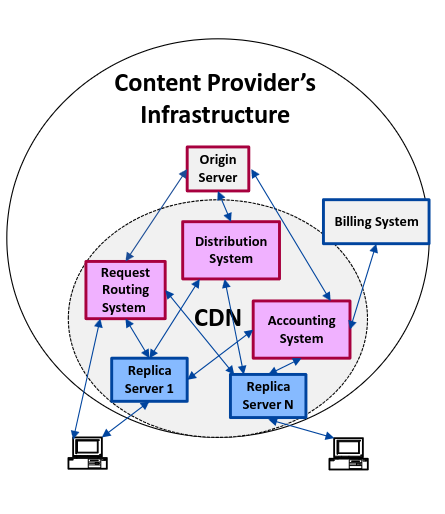
\includegraphics[width=0.5\textwidth]{pictures/7/architettura.png}
	\caption{Esempio di architettura di una CDN.}
\end{figure}
\section{Sistema di request routing e DNS}
Il Domain Name System (DNS) è usato per instradare una richiesta da un client a uno specifico server replica della CDN.
\\
Meccanismi alternativi:
\begin{itemize}
	\item \textbf{DNS redirection}
	\item \textbf{URL rewriting}
\end{itemize}\newpage
\begin{multicols}{2}
	\begin{center}
		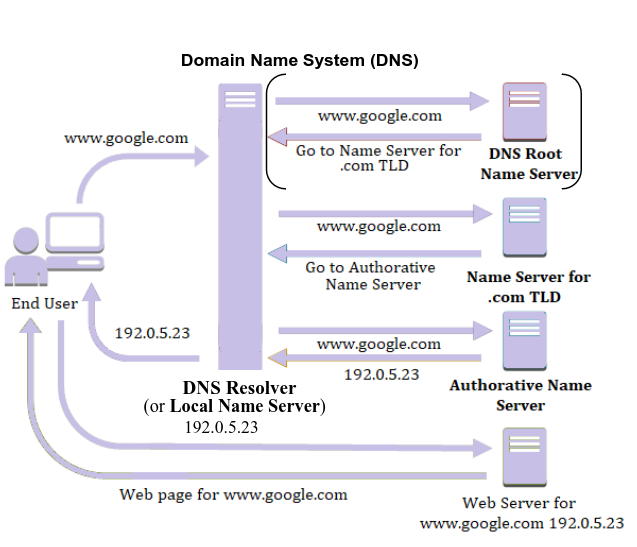
\includegraphics[width=\linewidth]{pictures/7/dns.png}
	\end{center}
	\columnbreak
	\begin{center}
		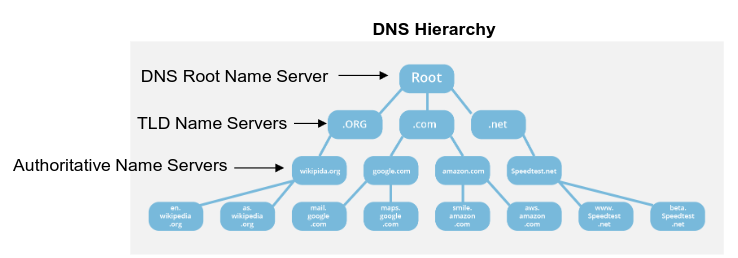
\includegraphics[width=\linewidth]{pictures/7/gerarchiadns.png}
	\end{center}
	
\end{multicols}
\subsection{DNS redirection}
L'Authoritative Name Server può:
\begin{enumerate}
	\item delegare la risoluzione del nome host a un name server controllato dalla CDN;
	\item risolvere direttamente l'hostname puntando a una cache CDN.
\end{enumerate}
\begin{figure}[H]
	\centering
	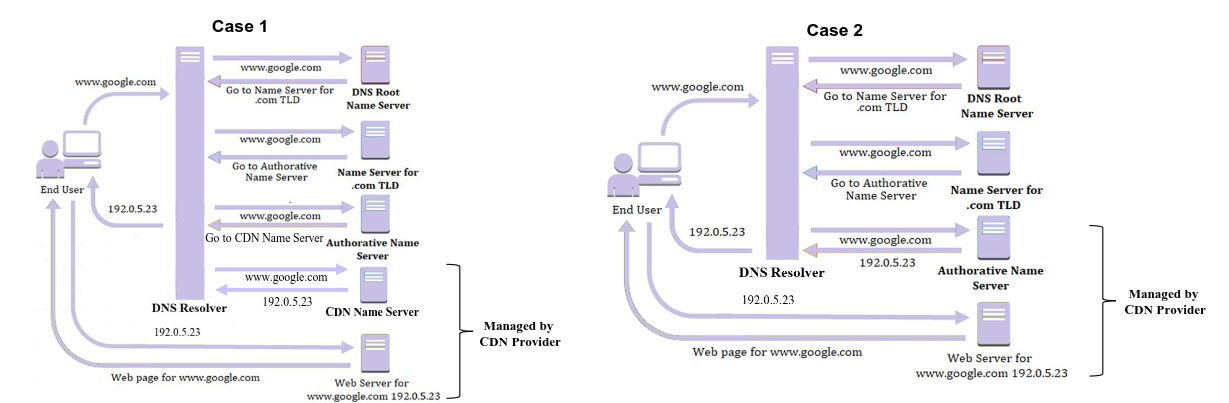
\includegraphics[width=\textwidth]{pictures/7/dnsredirection.png}
	\caption{Esempio di DNS redirection.}
\end{figure}
Il secondo caso è possibile solo se il CDN Provider può gestire l'Authoritative Name Server, previo accordo con il Content Provider.

\subsection{URL rewriting}
Il Content Provider riscrive gli URL nella pagina HTML per specificare quali oggetti embedded devono essere recuperati tramite CDN (tipicamente contenuti statici).
\\
Esempio:
\begin{verbatim}
https://my.origin-domain.com/path/to/img.jpg
-> https://my.cdn-domain.com/path/to/img.jpg
\end{verbatim}
\noindent
Per ogni oggetto embedded viene effettuata una risoluzione hostname specifica.
\\
Diversamente dal DNS redirection, nella risoluzione dei nomi il Content Provider viene bypassato: la risoluzione avviene direttamente tramite la CDN.
\\
Nota: oggetti embedded della stessa pagina possono essere recuperati da replica server diversi.

\section{Esempio di CDN: Akamai}
Akamai è un'azienda statunitense che fornisce diversi servizi Internet.
\begin{itemize}
	\item Fondata nel 1998 in Massachusetts.
	\item Leader mondiale tra i CDN Provider in termini di volume di traffico.
\end{itemize}
\noindent
Akamai dispone di una delle CDN piu diffuse al mondo. Molti Content Provider usano la CDN di Akamai per distribuire contenuti; tra i partner commerciali sono citate aziende come Apple, Facebook e Google.

\subsection{Architettura Akamai}
\begin{figure}[H]
	\centering
	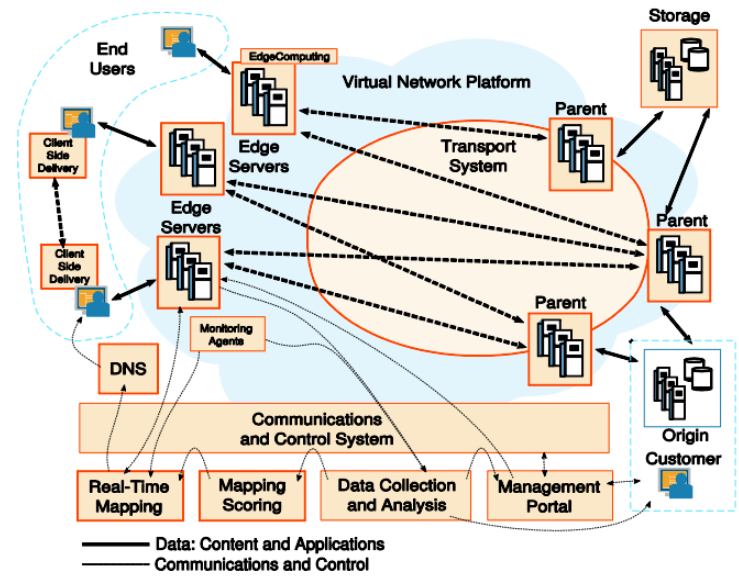
\includegraphics[width=0.8\textwidth]{pictures/7/architetturaAkamai.png}
	\caption{Esempio di architettura di Akamai.}
\end{figure}
L'architettura di Akamai segue tutti i principi introdotti fino ad ora:
\begin{itemize}
	\item componenti per gestione di distribuzione contenuti, instradamento delle richieste e accounting;
	\item corrispondenza terminologica: \texttt{Parent} $\rightarrow$ reverse proxy (replica server), \texttt{Edge Server} $\rightarrow$ forward proxy (replica server).
\end{itemize}

\subsection{Akamai: URL rewriting e routing}
Un Content Provider che vuole distribuire parte dei propri contenuti (ad esempio oggetti embedded di un sito) tramite Akamai deve rinominare gli URL di tali contenuti con un prefisso specifico:
\begin{itemize}
	\item \textbf{Akamai Resource Locator (ARL)}.
\end{itemize}
\noindent
La risoluzione dell'hostname verso l'indirizzo IP di un server replica Akamai è svolta dal DNS Akamai.
\\
Il server replica selezionato deve essere:
\begin{itemize}
	\item vicino al client;
	\item non sovraccarico.
\end{itemize}
\noindent
Akamai esegue misure e test per monitorare continuamente lo stato della rete e dei server replica. In questo modo, il DNS puo determinare il server replica ottimale da cui recuperare il contenuto richiesto da uno specifico utente.
\subsection{Akamai Resource Locator (ARL)}
Esempio di ARL:
\begin{verbatim}
http://a212.g.akamai.net/7/620/16/259fdbf4ed29de/news.bbc.co.uk/i/22.gif
\end{verbatim}
\noindent
Parti dell'ARL:
\begin{itemize}
	\item Host Part: \texttt{a212.g.akamai.net}
	\item Akamai Control Part: \texttt{/7/620/16/259fdbf4ed29de/}
	\item Content URL: \texttt{news.bbc.co.uk/i/22.gif}
\end{itemize}
\noindent
Akamai fornisce al Content Provider uno strumento che trasforma un URL originario (es. \texttt{news.bbc.co.uk/i/22.gif}) nell'ARL.
\\
In questo modo, il client accede ad Akamai (es. \texttt{a212.g.akamai.net}) e non all'origin server.

\subsection{Akamai: DNS redirection a due livelli}
Akamai adotta due livelli di DNS redirection:
\begin{enumerate}
	\item \textbf{Akamai Top-Level Name Server (TLNS)}
	\begin{itemize}
		\item Localizzazione: 4 core node negli USA, 3 in Europa, 1 in Asia (TLNS originale), piu molti cluster globali aggiunti successivamente.
		\item I TLNS rispondono indicando un LLNS scelto da un insieme di 8 LLNS vicini all'utente.
	\end{itemize}
	\item \textbf{Akamai Low-Level Name Server (LLNS)}
	\begin{itemize}
		\item Puntano agli Akamai Edge Server che consegnano i contenuti.
		\item Eseguono load balancing.
	\end{itemize}
\end{enumerate}

\subsection{Esempio di DNS redirection a due livelli in Akamai}
L'esempio mostrato nelle slide e compatibile con il \emph{Caso 1} della DNS redirection (delegare la risoluzione al name server della CDN), con una differenza: nel dominio CDN la risoluzione avviene su due livelli (TLNS + LLNS).
\\
Se viene usato URL rewriting, alcuni passaggi della risoluzione DNS vengono saltati (passi 4-5-6-7 nell'esempio in slide):
\begin{itemize}
	\item nessuna DNS redirection intermedia;
	\item risoluzione piu veloce.
\end{itemize}
\begin{figure}[H]
	\centering
	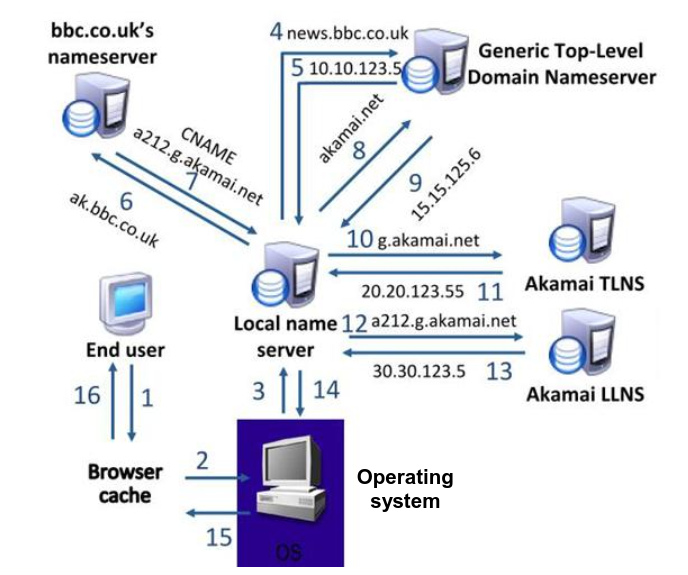
\includegraphics[width=0.8\textwidth]{pictures/7/redirection.png}
	\caption{Esempio di DNS redirection a due livelli in Akamai.}
\end{figure}